The pruning strategy is a key for the accuracy and efficiency of root cause localization.
We evaluate the effect of the pruning strategy by analyzing how the accuracy and time of root cause localization change with the threshold of correlation coefficient.
To this end, we run \app~to analyze the 75 availability issues with different threshold settings and measure the accuracy and time.
We choose the top-3 hit ratio (i.e., HR@3) as the indicator of accuracy.

The results of the evaluation are shown in Figure~\ref{fig:rq3}.
It can be seen that both the accuracy and time decrease with the increase of the threshold, as more services and service call edges are pruned in the analysis process and less services are reached and considered.
It can also be seen that the accuracy remains 0.67 when the threshold increases from 0 to 0.7, while the time decreases from 75 seconds to 46 seconds.
This analysis confirms the effectiveness of the pruning strategy, which can significantly improve the efficiency of root cause localization while keeping the accuracy.
And the best threshold is 0.7 for these availability issues.

\begin{figure}[ht]
	\centering
	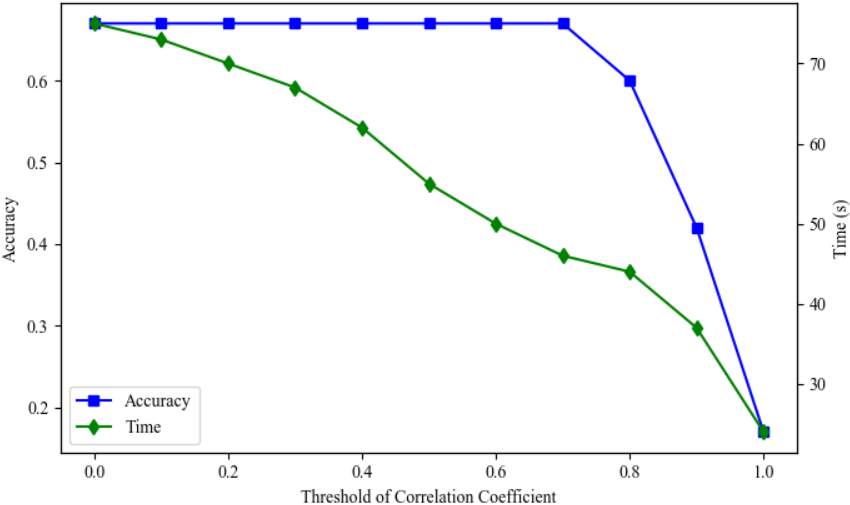
\includegraphics[width=0.5\textwidth]{images/pruningEffect.png}
	\vspace{-8pt}
	\caption{Evaluation of the Effect of the Pruning Strategy}\label{fig:rq3}
	\vspace{-10pt}
\end{figure}

